\documentclass[tikz,border=5pt]{standalone}
\usepackage{tikz}
\usetikzlibrary{calc}

\begin{document}
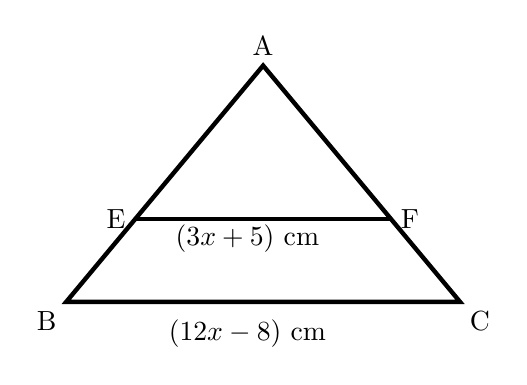
\begin{tikzpicture}

% Define vertices of triangle
\coordinate (A) at (2.5, 3);
\coordinate (B) at (0, 0);
\coordinate (C) at (5, 0);

% Points E and F on sides AB and AC (approximately 35% from B and C)
\coordinate (E) at ($(A)!0.65!(B)$);
\coordinate (F) at ($(A)!0.65!(C)$);

% Draw triangle ABC
\draw[ultra thick] (A) -- (B) -- (C) -- cycle;

% Draw line EF
\draw[ultra thick] (E) -- (F);

% Labels for vertices
\node[above] at (A) {A};
\node[below left] at (B) {B};
\node[below right] at (C) {C};
\node[left] at (E) {E};
\node[right] at (F) {F};

% Length labels
\node at (2.3, 0.8) {$(3x + 5)$ cm};
\node at (2.3, -0.4) {$(12x - 8)$ cm};

\end{tikzpicture}
\end{document}